\section{Difference between fundamental and applied linear algebra. Problems with the real data. Pseudoinverse matrices. Skeletonization.}
    \par 
    Let's consider some of the standard linear algebra problems, for example, solving the systems of linear equations. It can be written:
    \[
        A\vec{x} = \vec{b},    
    \]
    where $A = M_{m \times n}(F)$ -- the matrix of coefficients, $\vec{x} = \begin{bmatrix}
        x_1 \\
        \vdots \\
        x_n
    \end{bmatrix} \in F^n$ -- unknown vector and $\vec{b} \in F^m$ -- known vector. Solving such systems is our goal. In the best situation we can write out the solution:
    \[
        \vec{x} = A^{-1}\vec{b}.
    \]
    Or we have another method in a more general situation, when the matrix of the coefficients can be rectangular or degenerate, not inverted. We can provide Gaussian elimination:
    \[
        \scalebox{1.5}{$[A | b] \overset{\text{Gaussian}}{ \underset{\text{elimination}}{\xymatrix@C=3em{{}\ar@{~>}[r]&{}}}}$}
        \left[\begin{tabular}{clp{0.1cm}p{0.1cm}l}
            \multicolumn{1}{l}{\scalebox{1.25}{$1$}}        &         &\multicolumn{1}{l}{\multirow{2}{*}{\scalebox{2.5}{$\mathlarger{*}$}}}  & \multicolumn{1}{c|}{} & \scalebox{1.25}{$b_1$}    \\
\multicolumn{1}{l}{}         & \scalebox{1.25}{$1$}       & \multicolumn{1}{c}{} & \multicolumn{1}{c|}{}                   & \scalebox{1.25}{$b_2$}    \\
            \multicolumn{2}{c}{\multirow{2}{*}{
                
\begin{tikzpicture}[x=0.75pt,y=0.75pt,yscale=-1,xscale=1]
                    \draw  [line width=1.75]  (304.32,138.5) .. controls (312.66,138.5) and (319.43,147.68) .. (319.43,159) .. controls (319.43,170.32) and (312.66,179.5) .. (304.32,179.5) .. controls (295.98,179.5) and (289.21,170.32) .. (289.21,159) .. controls (289.21,147.68) and (295.98,138.5) .. (304.32,138.5) -- cycle ;
                    \end{tikzpicture}
            }} & \scalebox{1.25}{$\ddots$}              & \multicolumn{1}{l|}{}  & \scalebox{1.25}{$\vdots$} \\
            \multicolumn{2}{c}{}                   &                       & \multicolumn{1}{l|}{\scalebox{1.25}{$1$}} & \scalebox{1.25}{$b_r$}    \\[0.05cm]
            % \multicolumn{5}{c}{\resizebox{85pt}{25pt}{\rotatebox{90}{$0$}}}    
            \multicolumn{5}{c}{
\begin{tikzpicture}[x=0.75pt,y=0.75pt,yscale=-1,xscale=1]
                \draw [line width=1.75]  (246,143.5) .. controls (246,133.56) and (273.41,125.5) .. (307.21,125.5) .. controls (341.02,125.5) and (368.43,133.56) .. (368.43,143.5) .. controls (368.43,153.44) and (341.02,161.5) .. (307.21,161.5) .. controls (273.41,161.5) and (246,153.44) .. (246,143.5) -- cycle ;
                \end{tikzpicture}
                }                                                                        
            \end{tabular}\right]
    \]
    After that we can easily express one variable in terms of another one step by step.
    \par
    But in the real world with the linear models, the initial data can be inaccurate due to the observational errors in some physical cases or human reliability in, for example, social or business situations. It can lead to some problems. For example, in Gaussian elimination, you need to choose a pivot variable, and if it contains some errors, then other computations will increase them. In situations with high order errors, such methods cannot be applied. But even if you have the exact formula and enough resources for calculating the inverted matrix, you will realize that the inverse is obtained with some errors. Another problem is rounding. It happens because of the precise nature of Gaussian elimination algorithm or other algorithms and machine precision. It is hard and slow to calculate the precision of the solution.
    \par
    The next problem is about speed or complexity of calculations. For example, the complexity for Gaussian elimination is $\bigO(n^3)$. It is not suitable for dealing with, for example, video or signals in real time.
    \par 
    Suppose you have created a linear model that more or less describes the production or business process. For example, you get the vector of unknowns $\vec{x}$, which means that you should sell $x_1$ copies of product 1 and $x_2$ copies of product 2, etc. How much must you produce or sell? It is a set of possible scenarios needed to solve. Then you can face an indefinite system because your initial data are not exact.
    \subsubsection*{Indefinite (indeterminate) system}
    For example, it means system with less equations than variables or linearly dependent equations. It can be some system of a kind:
    \[
        \left\{ \begin{array}{c}
            x_1 + 2x_2 = 3,\\
            2x_1 + 4x_2 = 5
        \end{array}
            \right.  
    \]
    So we have two lines of the same kind. The problem is how to pick one value of the vector $\vec{x}$. 
    \begin{wrapfigure}[12]{l}{0.5\columnwidth}
        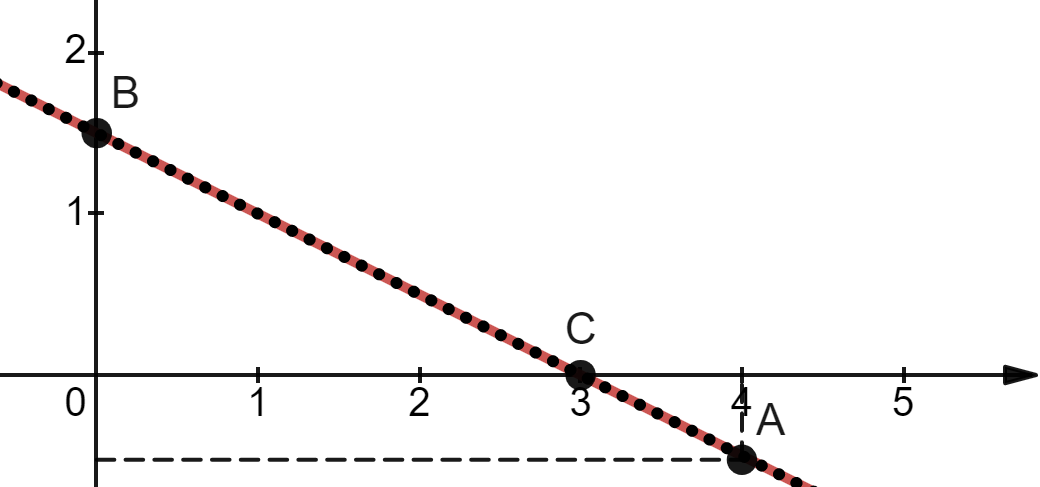
\includegraphics[height=0.235\columnwidth, width=0.5\columnwidth]{lectures/images/indefinite_system.png}
        \caption*{\scriptsize{Example of indefinite system.}}
        \label{fig:indefinite_system}
    \end{wrapfigure}
    Mathematically, we can pick every point from this line, but, for example, negative values (point A), obviously looks strange or even inappropriate for our case. Or, for example, you can pick either point B, or C. Again, mathematically there are solutions of our systems, but it can be no optimum solution. We will understand it on the next lecture. Another problem is about inconsistent system if there is no set of values for the unknown vector $\vec{x}$ that satisfies all of the equations. Or in mathematical terms, it happens when rank of initial coefficients matrix is less than rank of augmented matrix (a matrix of a kind $[A|b]$). Such systems can be either determined (defined) or underdetermined.
    \subsubsection*{Inconsistent system}
    \begin{wrapfigure}[12]{r}{0.24\columnwidth}
        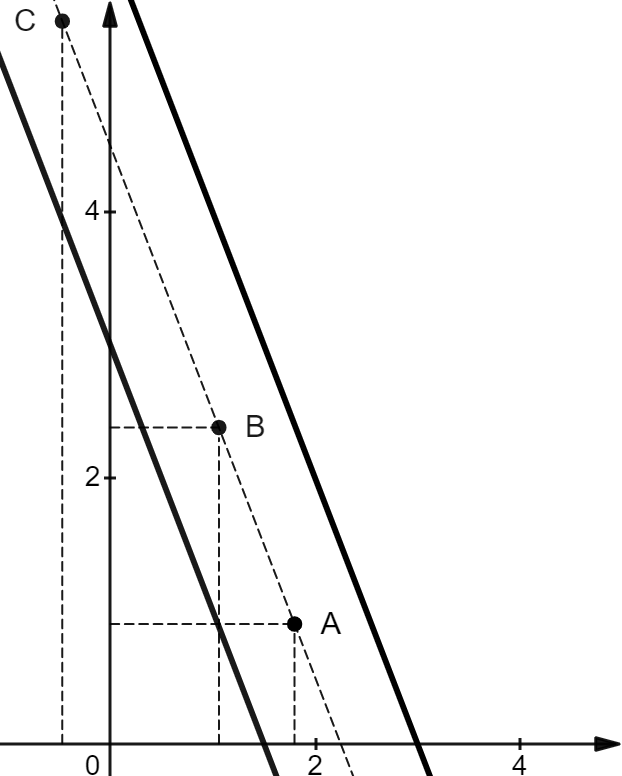
\includegraphics[height=0.3\columnwidth, width=0.24\columnwidth]{lectures/images/inconsistent_system_without_vectors.png}
        \caption*{\scriptsize{Example of inconsistent system.}}
        \label{fig:inconsistent}
    \end{wrapfigure}
    For example, you have approximately calculated several coefficients of the initial matrix and after the approximate calculations you obtained the system of equations, for example, a kind of: 
    \[
        \left\{ \begin{array}{c}
        x_1 + 2x_2 = 3,\\
        2x_1 + 4x_2 = 5
           \end{array}
        \right. 
    \]
    It looks like 2 parallel lines. Of course, rarely some $\vec{x}$ exists, but we cannot solve this system because the coefficients are not exact (they contain some random errors, rounding after calculations, etc.). But answers can still be the same. How much do we need to sell? We can choose, for example, solutions A or B or even C, but what would be more optimal or correct. We will give an answer to this question right off the bat in the next lecture. Now let's define some new concepts that will help us with it.
    \subsection*{Pseudoinverse Matrices}
    \begin{definition}{Pseudoinverse}{}
        Let $A \in M_{m\times n}(\C)$. Then $C$ is called pseudoinverse matrix to A, or Moore-Penrose (pseudo) inverse, if it is satisfies Penrose axioms: 
        \begin{center}
            \renewcommand{\arraystretch}{1.2}
            \setlength\arrayrulewidth{1.25pt}
            \begin{tabular}{p{9cm}|p{8cm}}
                \cline{2-2}
                \vspace*{-0.8cm}
                \begin{enumerate}[I.]
                    \itemsep-0.5em
                    \item $ACA = A$;
                    \item $CAC = C$;
                    \item $(AC)^* = AC$;
                    \item $(CA)^* = CA$.
                \end{enumerate}
                &Notation: $C = A^+$.
                \end{tabular}
        \end{center} 
    \end{definition}
    \begin{note}{}{}
        If $A \in M_{m\times n} (\C)$, then $C \in M_{n\times m}(\C)$.
    \end{note}
    \begin{note}{}{}
        if $A \in M_{n\times n}, \det A \neq 0$, then $A^{-1}$ is a pseudoinverse.
    \end{note}
    \begin{proposition}{}{}
        If a pseudoinverse matrix $C$ to $A$ exists, it is unique.
    \end{proposition}
    \begin{proof}
        Suppose $B$ is some another pseudoinverse matrix to $A$. Then:
        \begin{gather*}
            AB \overset{\rom{1}}{=} \left(AC \right)\left(AB\right) \overset{\rom{3}}{\Rightarrow} \left(AC \right)^*\left(AB\right)^* \Rightarrow C^*\left(A^*B^*A^*\right) = C^*(ABA)^* = (AC)^* = AC.
        \end{gather*}
        Similarly, $BA=CA$. Now, $B\overset{\rom{2}}{=} BAB = BAC = CAC = C$.
    \end{proof}\\
    \Ex $A = O_{m\times n} = \begin{bmatrix}
        0 & \ldots & 0\\
        \vdots & \ddots & \vdots\\
        0 & \ldots & 0
    \end{bmatrix}$, then $A^+ = O_{n\times m}$.\\
    \Ex $\begin{bmatrix}
        5 & 0 \\
        0 & 0 \\
        0 & 0
    \end{bmatrix}^+ = \displaystyle\begin{bmatrix}
        \medmath{\frac{1}{5}} & 0 & 0\\
        0 & 0 & 0
    \end{bmatrix}$.\\
    \Ex $\begin{bmatrix}
        1 \\ 2
    \end{bmatrix}^+ = \begin{bmatrix}
        \medmath{\frac{1}{5}} & \medmath{\frac{2}{5}}
    \end{bmatrix}$.\\
    \Ex Let $A = \vec{a} \in \C^n$, then
    \[\vec{a}^{\, +} = \dfrac{1}{a^*a}\vec{a}^{\, *} 
                     = \dfrac{1}{|\vec{a}\,|^2}\vec{a}^{\, *}
                     = \dfrac{1}{|a_1|^2 + \ldots + |a_n|^2} \vec{a}^{\, *}.\]
    \begin{proposition}{}{}
        Suppose that $A \in M_{m\times n}(\C)$ has full column rank, that is, $\rank A = n$. Then
        $A^+ = (\underbrace{A^*A}_{n\times n})^{-1}A^*.$
    \end{proposition}
    \begin{proposition}{}{}
        Suppose that $A \in M_{m\times n}(\C)$ has full row rank, that is, $\rank A = m$. Then $A^+ = A^* (\underbrace{AA^*}_{m\times m})^{-1}.$
    \end{proposition}
    \Exc{Check \rom{1}-\rom{4} axioms for these $A^+$.}
    
    \begin{definition}{Skeletonization}{}
        A full rank decomposition (or skeletonization) of a matrix $A \in M_{m\times n}(\C)$ with $r = \rank A$ is a decomposition:
        \[
            A = F \cdot G, \hspace*{0.5cm} \begin{aligned}
                F\ \in \ M_{m\times r}(\C),\\
                G\ \in \ M_{r\times n}(\C).
            \end{aligned}  
        \]
        Then $\rank F = \rank G = r$. $F, G$ are called matrices of full rank.
    \end{definition}
    \begin{theorema}{}{}
        For each matrix $A \in M_{m\times n}(\C)$, its pseudoinverse matrix $A^+$ exists. If $A = F \cdot G$ is a full rank decomposition, then
        \[
            A^+ = G^+F^+ = G^*\left(G,G^*\right)^{-1} \left(F^*, F\right)^{-1}F^*. 
        \]
    \end{theorema}